\chapter{Introduction}
\label{ch:Intro}

The Standard Model (SM) \cite{gaillard_standard_1999} is a robust framework that allows for accurate predictions of processes involving the interactions of elementary particles. It has been developed over the course of many decades, which involved many additions such as three generations of quarks and leptons and the combination of Electromagnetism and the Weak force into a single theory. Unfortunately, we have observation for phenomena that is not explained by the SM and has eluded physicists. We present a search for a potential particle beyond the SM.
\section{Motivation}
\label{sec:Motivation}

Through various methods of experiment, we have seen that the elementary particles in the SM does not explain all of the known matter in the universe. From galactic velocity rotational curves we can deduce that the mass of galaxies must be much more than the visible matter that can be measuredmust act quite weakly with the three forces of the SM, but can still be important for gravitational effects. There are many theories beyond the SM that can explain these effects, but we will concentrate on Supersymmetry (SUSY) \cite{ramond_dual_1971, volkov_possible_1972, wess_supergauge_1974, fayet_supergauge_1975, barbieri_gauge_1982, chamseddine_locally_1982, hall_supergravity_1983, kane_study_1994, papucci_natural_2012} because of the potential for a dark matter candidate \cite{feng_dark_2010, bertone_dark_2005}, a solution to the hierarchy problem, and a potential Grand Unified Theory (GUT) \cite{georgi_unity_1974, georgi_hierarchy_1974, buras_aspects_1978}.

\begin{figure}
 	\centering
	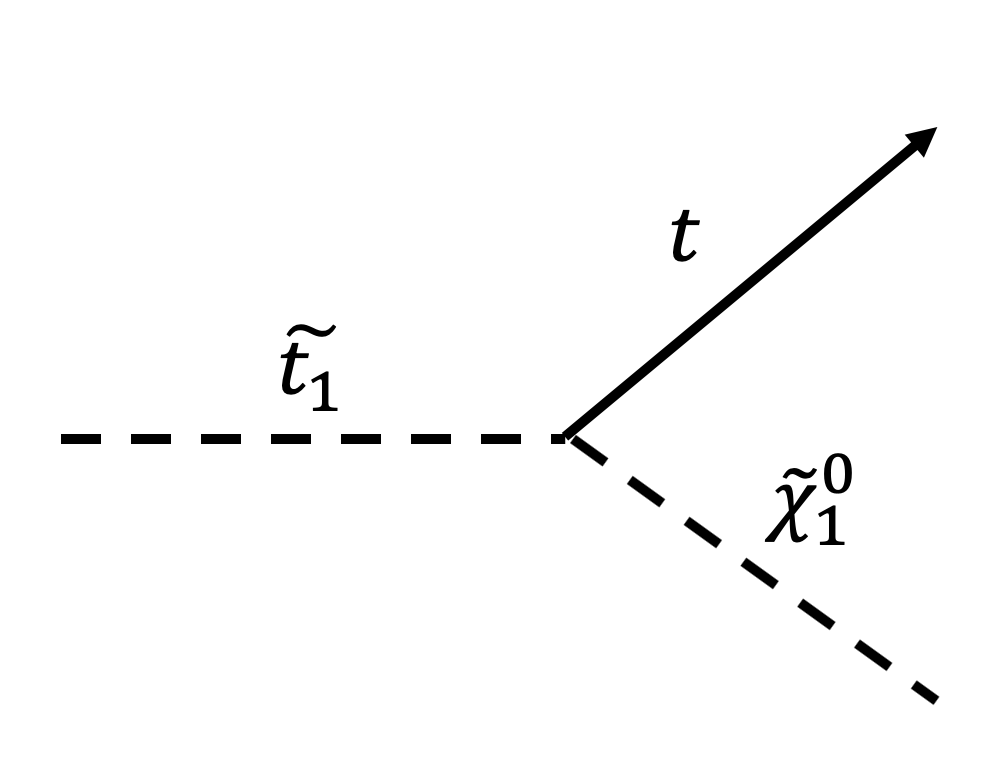
\includegraphics[width=0.65\textwidth]{topSquarkDecay.png}
 	\caption[Top Squark Decay]{The decay of a top squark to a top quark and a neutralino.}
 	\label{topSquarkDecay} 
\end{figure}

SUSY allows for every fermion to have a bosonic partner, and vice-versa, which has all of the same quantum numbers except for a difference of $\frac{1}{2}$-integer spin. We know that since it has not yet been found that the theory must be a broken symmetry, such that the masses of the SUSY partners must have a higher mass than the SM particle. One of the main aspects of simplified SUSY, is the conservation of $R$-parity, which implies the existence of a Lightest Supersymmetric Particle (LSP). There are other models with $R$-parity violating decays \cite{barbier_r-parity-violating_2005, grossman_sneutrino_1999}, but we are not considering them. This LSP could be a potential dark matter candidate since it is stable and weakly interacting. We are interested in the neutralino, \neutralino, as the LSP, see Fig. \ref{topSquarkDecay}. 

\begin{figure}
 	\centering
	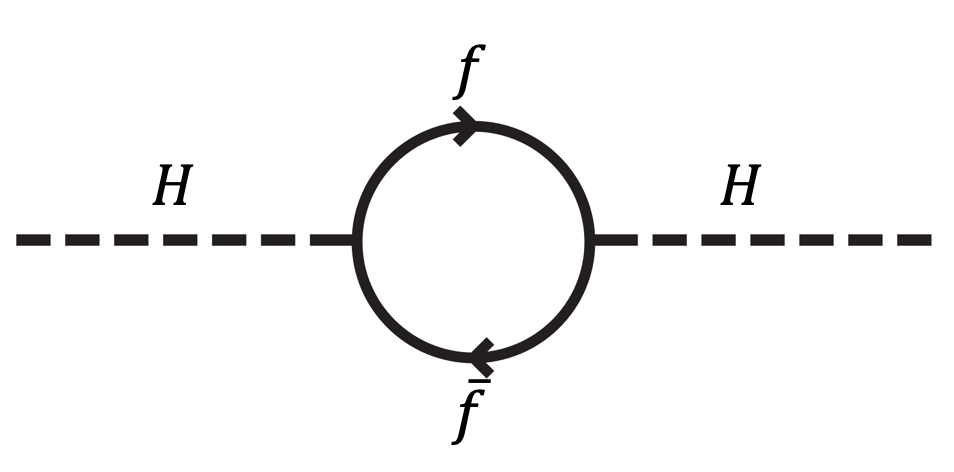
\includegraphics[width=0.65\textwidth]{HierarchyFermionLoop.png}
 	\caption[Hierarchy Fermion Loop]{The loop corrections to the Higgs boson interacting with a fermion. This is a next-to-leading order (NLO) correction to the Higgs boson mass.}
 	\label{HierarchyFermion} 
\end{figure}

The hierarchy problem is due to the loop interactions of massive quarks with the Higgs boson. This coupling causes a quadratic divergence of the Higgs mass, $m_H$, and can only be renormalized by fine tuning the coupling parameters, see Fig. \ref{HierarchyFermion}. The divergence is cutoff at the planck mass, $m_P$, known as the ultraviolet cutoff. A potential solution is the coupling of an additional bosonic particle to the quarks. This additional coupling allows for a cancellation of quadratic divergence into a logarithmic divergence, which is then renormalizable by the normal methods. This can renormalize the mass of the Higgs boson to the measured value of $m_H=125.18$ GeV \cite{chatrchyan_observation_2012, aad_observation_2012, chatrchyan_observation_2013, atlas_collaboration_combined_2015} that was discovered in 2012. Finally, SUSY also allows for a mechanism for a potential GUT. The additional superpartners allow for the three forces of the SM to converge at a large energy scale of the order $10^{16}$ GeV. We now need to develop a search strategy to try and detect these potential SUSY particles.

\section{Search}
\label{sec:search}

There are many possible searches for SUSY particles. In the Minimal Supersymmetric Standard Model (MSSM) \cite{martin_supersymmetry_1997}, it can be determined that the lightest squark that can be produced at the Large Hadron Collider (LHC) is the top quark, \st{}, which will then decay into SM particles and the LSP.  We are developing an all-hadronic search to find the \st{} which will be as inclusive as possible, so we will include all possible decay modes to get additional limits or possible detection. 

Due to the all hadronic aspect of the decay, the main backgrounds are caused by a lost lepton due to a lepton being missed for various reasons, \Znunu{} background where the missing energy is caused by the neutrinos escaping the detector, Quantum Chromodynamics (QCD) background which can be caused by the mis-measurement of jets in the event, and a rare background caused by many different types of processes which are estimated by a three lepton method of identification. We have developed 183 search regions to look for the top squark, \st{}. This is then used to get a statistical estimation of the sensitivity on the cross section for each of the production processes that we include in search. In the following chapters, we will: look into the derivation of the SM and motivations for SUSY; provide a description of the Compact Muon Solenoid (CMS) detector and the various subdetectors; describe the object selection and search strategy for the analysis; predict background estimations for each individual background; and give a description and analysis of the results and limits. 

